% Algebra 2 Lesson 2-5 fast-track packet: Completing the Square (enVision A2, Example 3 only; brief lesson)
% Quiz map (2-5 Lesson Quiz, a2_2-5_TE.tex): item 1 -> Example 1 (cut; the square-root step of Example 3);
% item 2 -> Example 2B (cut; the first three lines of Example 3); items 3 and 5 -> Example 3 (kept);
% item 4 -> Example 4 (cut; left off the short-form quiz). Item 5 needs "divide by a first": Practice block (R5).
% DOK 3: Practice & Problem Solving 16 (Example 3, Construct Arguments) is the Exit question.
% Shared preamble for the "fast" (hacked-down) Algebra 2 lesson packets, Oct 2026.
% Each packet: % Shared preamble for the "fast" (hacked-down) Algebra 2 lesson packets, Oct 2026.
% Each packet: % Shared preamble for the "fast" (hacked-down) Algebra 2 lesson packets, Oct 2026.
% Each packet: \input{fast-packet-template} then \begin{document} ... \end{document}.
\documentclass[12pt]{article}
\usepackage[margin=0.7in]{geometry}
\usepackage{amsmath,amssymb}
\usepackage{booktabs,tabularx,array}
\usepackage{enumitem}
\usepackage[T1]{fontenc}
\usepackage[utf8]{inputenc}
\usepackage{lmodern}
\usepackage{tikz}
\usepackage{pgfplots}
\pgfplotsset{compat=1.18}
\usepackage{xcolor}
\setlist{nosep,leftmargin=1.4em}
\setlength{\parindent}{0pt}
\setlength{\parskip}{6pt}
\renewcommand{\arraystretch}{1.35}
\newcolumntype{Y}{>{\raggedright\arraybackslash}X}
\pagestyle{empty}

% blanks and workspace
\newcommand{\blank}[1][2.6cm]{\rule[-2pt]{#1}{0.5pt}}
\newcommand{\lines}[1][1]{\par\vspace{2pt}\foreach \i in {1,...,#1}{\rule{0pt}{22pt}\rule{\linewidth}{0.4pt}\par}}
\newcommand{\wspart}[2]{\vspace{4pt}{\large\bfseries #1: #2}\par\vspace{-6pt}\rule{\textwidth}{0.4pt}\par}

% header: \packethead{Lesson 1-3}{Piecewise-Defined Functions}
\newcommand{\packethead}[2]{%
{\LARGE\bfseries #2}\hfill Name \blank[5cm]\\[2pt]
Algebra 2 \quad #1 (fast track) \hfill Date \blank[2.5cm] \quad Period \blank[1.2cm]\par\vspace{2pt}}

% boxed goals: \goals{learning goal}{language goal}
\newcommand{\goals}[2]{%
\fbox{\parbox{\dimexpr\textwidth-2\fboxsep-2\fboxrule}{%
\textbf{Learning goal:} #1\\[2pt]
\textbf{Language goal:} #2}}\par}

% quiz target box: \quiztarget{text}
\newcommand{\quiztarget}[1]{%
\vspace{4pt}\colorbox{gray!12}{\parbox{\dimexpr\textwidth-2\fboxsep}{\textbf{On the quiz:} #1}}\par}

% IXL table row helper: code & skill & which quiz question it feeds
\newcommand{\ixlrow}[3]{\texttt{#1} & #2 & #3 \\}

% one grid style for every graph; override xmin/xmax/... per plot
\pgfplotsset{sheetgrid/.style={
  axis lines=middle, grid=both, grid style={gray!45},
  xmin=-10.5, xmax=10.5, ymin=-10.5, ymax=10.5,
  xtick={-10,-8,...,10}, ytick={-10,-8,...,10},
  x=0.28cm, y=0.28cm,
  ticklabel style={font=\scriptsize, fill=white, inner sep=1pt},
  xlabel={$x$}, ylabel={$y$},
  axis line style={thick}, clip=true}}
% unit grid for small windows
\pgfplotsset{unitgrid/.style={sheetgrid,
  xmin=-5.5, xmax=5.5, ymin=-5.5, ymax=5.5,
  xtick={-5,...,5}, ytick={-5,...,5}, x=0.5cm, y=0.5cm}}
% open and closed endpoints
\tikzset{closed/.style={circle, fill, inner sep=1.6pt},
         open/.style={circle, draw, fill=white, inner sep=1.4pt}}
 then \begin{document} ... \end{document}.
\documentclass[12pt]{article}
\usepackage[margin=0.7in]{geometry}
\usepackage{amsmath,amssymb}
\usepackage{booktabs,tabularx,array}
\usepackage{enumitem}
\usepackage[T1]{fontenc}
\usepackage[utf8]{inputenc}
\usepackage{lmodern}
\usepackage{tikz}
\usepackage{pgfplots}
\pgfplotsset{compat=1.18}
\usepackage{xcolor}
\setlist{nosep,leftmargin=1.4em}
\setlength{\parindent}{0pt}
\setlength{\parskip}{6pt}
\renewcommand{\arraystretch}{1.35}
\newcolumntype{Y}{>{\raggedright\arraybackslash}X}
\pagestyle{empty}

% blanks and workspace
\newcommand{\blank}[1][2.6cm]{\rule[-2pt]{#1}{0.5pt}}
\newcommand{\lines}[1][1]{\par\vspace{2pt}\foreach \i in {1,...,#1}{\rule{0pt}{22pt}\rule{\linewidth}{0.4pt}\par}}
\newcommand{\wspart}[2]{\vspace{4pt}{\large\bfseries #1: #2}\par\vspace{-6pt}\rule{\textwidth}{0.4pt}\par}

% header: \packethead{Lesson 1-3}{Piecewise-Defined Functions}
\newcommand{\packethead}[2]{%
{\LARGE\bfseries #2}\hfill Name \blank[5cm]\\[2pt]
Algebra 2 \quad #1 (fast track) \hfill Date \blank[2.5cm] \quad Period \blank[1.2cm]\par\vspace{2pt}}

% boxed goals: \goals{learning goal}{language goal}
\newcommand{\goals}[2]{%
\fbox{\parbox{\dimexpr\textwidth-2\fboxsep-2\fboxrule}{%
\textbf{Learning goal:} #1\\[2pt]
\textbf{Language goal:} #2}}\par}

% quiz target box: \quiztarget{text}
\newcommand{\quiztarget}[1]{%
\vspace{4pt}\colorbox{gray!12}{\parbox{\dimexpr\textwidth-2\fboxsep}{\textbf{On the quiz:} #1}}\par}

% IXL table row helper: code & skill & which quiz question it feeds
\newcommand{\ixlrow}[3]{\texttt{#1} & #2 & #3 \\}

% one grid style for every graph; override xmin/xmax/... per plot
\pgfplotsset{sheetgrid/.style={
  axis lines=middle, grid=both, grid style={gray!45},
  xmin=-10.5, xmax=10.5, ymin=-10.5, ymax=10.5,
  xtick={-10,-8,...,10}, ytick={-10,-8,...,10},
  x=0.28cm, y=0.28cm,
  ticklabel style={font=\scriptsize, fill=white, inner sep=1pt},
  xlabel={$x$}, ylabel={$y$},
  axis line style={thick}, clip=true}}
% unit grid for small windows
\pgfplotsset{unitgrid/.style={sheetgrid,
  xmin=-5.5, xmax=5.5, ymin=-5.5, ymax=5.5,
  xtick={-5,...,5}, ytick={-5,...,5}, x=0.5cm, y=0.5cm}}
% open and closed endpoints
\tikzset{closed/.style={circle, fill, inner sep=1.6pt},
         open/.style={circle, draw, fill=white, inner sep=1.4pt}}
 then \begin{document} ... \end{document}.
\documentclass[12pt]{article}
\usepackage[margin=0.7in]{geometry}
\usepackage{amsmath,amssymb}
\usepackage{booktabs,tabularx,array}
\usepackage{enumitem}
\usepackage[T1]{fontenc}
\usepackage[utf8]{inputenc}
\usepackage{lmodern}
\usepackage{tikz}
\usepackage{pgfplots}
\pgfplotsset{compat=1.18}
\usepackage{xcolor}
\setlist{nosep,leftmargin=1.4em}
\setlength{\parindent}{0pt}
\setlength{\parskip}{6pt}
\renewcommand{\arraystretch}{1.35}
\newcolumntype{Y}{>{\raggedright\arraybackslash}X}
\pagestyle{empty}

% blanks and workspace
\newcommand{\blank}[1][2.6cm]{\rule[-2pt]{#1}{0.5pt}}
\newcommand{\lines}[1][1]{\par\vspace{2pt}\foreach \i in {1,...,#1}{\rule{0pt}{22pt}\rule{\linewidth}{0.4pt}\par}}
\newcommand{\wspart}[2]{\vspace{4pt}{\large\bfseries #1: #2}\par\vspace{-6pt}\rule{\textwidth}{0.4pt}\par}

% header: \packethead{Lesson 1-3}{Piecewise-Defined Functions}
\newcommand{\packethead}[2]{%
{\LARGE\bfseries #2}\hfill Name \blank[5cm]\\[2pt]
Algebra 2 \quad #1 (fast track) \hfill Date \blank[2.5cm] \quad Period \blank[1.2cm]\par\vspace{2pt}}

% boxed goals: \goals{learning goal}{language goal}
\newcommand{\goals}[2]{%
\fbox{\parbox{\dimexpr\textwidth-2\fboxsep-2\fboxrule}{%
\textbf{Learning goal:} #1\\[2pt]
\textbf{Language goal:} #2}}\par}

% quiz target box: \quiztarget{text}
\newcommand{\quiztarget}[1]{%
\vspace{4pt}\colorbox{gray!12}{\parbox{\dimexpr\textwidth-2\fboxsep}{\textbf{On the quiz:} #1}}\par}

% IXL table row helper: code & skill & which quiz question it feeds
\newcommand{\ixlrow}[3]{\texttt{#1} & #2 & #3 \\}

% one grid style for every graph; override xmin/xmax/... per plot
\pgfplotsset{sheetgrid/.style={
  axis lines=middle, grid=both, grid style={gray!45},
  xmin=-10.5, xmax=10.5, ymin=-10.5, ymax=10.5,
  xtick={-10,-8,...,10}, ytick={-10,-8,...,10},
  x=0.28cm, y=0.28cm,
  ticklabel style={font=\scriptsize, fill=white, inner sep=1pt},
  xlabel={$x$}, ylabel={$y$},
  axis line style={thick}, clip=true}}
% unit grid for small windows
\pgfplotsset{unitgrid/.style={sheetgrid,
  xmin=-5.5, xmax=5.5, ymin=-5.5, ymax=5.5,
  xtick={-5,...,5}, ytick={-5,...,5}, x=0.5cm, y=0.5cm}}
% open and closed endpoints
\tikzset{closed/.style={circle, fill, inner sep=1.6pt},
         open/.style={circle, draw, fill=white, inner sep=1.4pt}}

\begin{document}

\packethead{Lesson 2-5}{Completing the Square}
\goals{I can solve quadratic equations by completing the square, even when the solutions are imaginary.}{I can explain each step of completing the square using the words perfect square trinomial, both sides, square root, and imaginary.}

\quiztarget{(1) Already a perfect square trinomial: take the square root of both sides (end of Example 3; full Savvas quiz only). (2) Bonus: write as $(x+p)^2=q$ (first three steps of Example 3). (3) Solve by completing the square; the solutions are imaginary (Example 3, Try It 3). (4) A rectangle from its perimeter and area (full Savvas quiz only). (5) Zeros when $x^2$ has a coefficient: divide by it, then Example 3 (Practice).}

\vspace{2pt}
\fbox{\parbox{\dimexpr\textwidth-2\fboxsep-2\fboxrule}{%
\begin{minipage}[c]{0.66\textwidth}
\textbf{Completing the square} is finding the number to add to $x^2+bx$ to make a \textbf{perfect square trinomial}.
That number is \textbf{half the coefficient of the middle term, squared}:
\[x^2+bx+\left(\tfrac{b}{2}\right)^2=\left(x+\tfrac{b}{2}\right)^2\]
\vspace{-12pt}

Example: $x^2+10x$. Half of 10 is 5, and $5^2=25$, so $x^2+10x+25=(x+5)^2$.
In an equation, add the number to \textbf{both sides} to keep it balanced.

\footnotesize Spanish: perfect square trinomial = \emph{trinomio cuadrado perfecto}; completing the square = \emph{completar el cuadrado}.
\end{minipage}\hfill
\begin{minipage}[c]{0.31\textwidth}
\centering
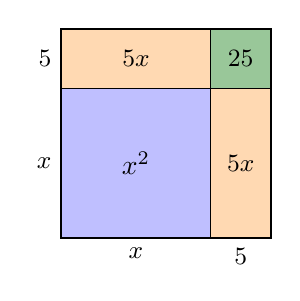
\begin{tikzpicture}[scale=0.95]
\fill[blue!25] (0,0) rectangle (2,2);
\fill[orange!30] (2,0) rectangle (2.8,2);
\fill[orange!30] (0,2) rectangle (2,2.8);
\fill[green!45!black!40] (2,2) rectangle (2.8,2.8);
\draw[thick] (0,0) rectangle (2.8,2.8);
\draw (2,0) -- (2,2.8); \draw (0,2) -- (2.8,2);
\node at (1,1) {$x^2$};
\node[font=\small] at (2.4,1) {$5x$};
\node[font=\small] at (1,2.4) {$5x$};
\node[font=\small] at (2.4,2.4) {$25$};
\node[font=\small, below] at (1,0) {$x$};
\node[font=\small, below] at (2.4,0) {$5$};
\node[font=\small, left] at (0,1) {$x$};
\node[font=\small, left] at (0,2.4) {$5$};
\end{tikzpicture}

{\scriptsize green 25 completes the square}
\end{minipage}}}

\wspart{Example 3}{Solve a Quadratic Equation by Completing the Square}
How can you solve $0=x^2-2x+3$ by completing the square?

{\renewcommand{\arraystretch}{1.15}
\begin{tabular}{@{\hspace{1.2em}}r@{\;}c@{\;}l@{\hspace{3.5em}}l@{}}
$0$ & $=$ & $x^2-2x+3$ & the equation \\
$-3$ & $=$ & $x^2-2x$ & move the constant: subtract 3 from both sides \\
$-3+1$ & $=$ & $x^2-2x+1$ & $b=-2$: $\bigl(\tfrac{-2}{2}\bigr)^2=1$; add 1 to \textbf{both sides} \\
$-2$ & $=$ & $(x-1)^2$ & write the perfect square trinomial as $(x-1)^2$ \\
$\pm\sqrt{-2}$ & $=$ & $x-1$ & take the \textbf{square root} of both sides ($\pm$) \\
$\pm i\sqrt{2}$ & $=$ & $x-1$ & $\sqrt{-2}=i\sqrt{2}$ \ (\textbf{imaginary}) \\
$1\pm i\sqrt{2}$ & $=$ & $x$ & add 1 to both sides
\end{tabular}\par}

\vspace{2pt}
The solutions of $0=x^2-2x+3$ are $x=1+i\sqrt{2}$ and $x=1-i\sqrt{2}$.

\textbf{Check} $x=1+i\sqrt2$: \ $(1+i\sqrt2)^2-2(1+i\sqrt2)+3=(-1+2i\sqrt2)-2-2i\sqrt2+3=0$ \checkmark

\textbf{Say it:} Half of $-2$, squared, is \blank[1.2cm], so $x^2-2x+1$ is a \blank[3.2cm]. I added it to both sides because \dots\ The square root of $-2$ makes the solutions imaginary because \dots
\lines[2]

\newpage

\wspart{Try It 3}{Solve by completing the square}
Solve the following equations by completing the square.

\begin{minipage}[t]{0.48\textwidth}
\textbf{a.} $0=x^2+4x+8$

\vspace{4pt}
Half of $b$, squared: \blank[2.4cm]
\lines[7]

\vspace{4pt}
$x=\blank[4.5cm]$
\end{minipage}\hfill
\begin{minipage}[t]{0.48\textwidth}
\textbf{b.} $0=x^2-8x+17$

\vspace{4pt}
Half of $b$, squared: \blank[2.4cm]
\lines[7]

\vspace{4pt}
$x=\blank[4.5cm]$
\end{minipage}

In part a, why is there an $i$ in the answer? Use the words \emph{square root} and \emph{imaginary}.\lines[2]

% R5 Practice: structural parallel of 2-5 Lesson Quiz item 5 (zeros of f(x) = -5x^2 + 4x - 1, a not 1, imaginary zeros); not the item itself.
\wspart{Practice}{When $x^2$ has a coefficient}
Find the zeros of the function $g(x)=-4x^2+8x-5$ by completing the square.

\textbf{Circle the coefficient of $x^2$.} It is not 1, so first set $g(x)=0$ and divide every term by it. Then complete the square as in Example 3.

\begin{minipage}[t]{0.55\textwidth}
\vspace{0pt}
$-4x^2+8x-5=0$

\vspace{2pt}
Divide by \blank[1cm]: \quad $x^2-\blank[1cm]x+\blank[1cm]=0$
\lines[5]
\end{minipage}\hfill
\begin{minipage}[t]{0.42\textwidth}
\vspace{0pt}
\fbox{\parbox{0.92\linewidth}{\centering
\vspace{4pt}
$x=\fbox{\rule{0pt}{14pt}\hspace{1.1cm}}+\fbox{\rule{0pt}{14pt}\hspace{1.1cm}}\,i$

\vspace{10pt}
$x=\fbox{\rule{0pt}{14pt}\hspace{1.1cm}}-\fbox{\rule{0pt}{14pt}\hspace{1.1cm}}\,i$
\vspace{4pt}}}

\vspace{6pt}
\small Why do the two zeros differ only in the sign of the $i$ part?
\lines[2]
\end{minipage}

\newpage

\wspart{IXL}{Practice for the quiz}
Go to IXL, Algebra 2. Type the code in the search box. Do the starred skills first.

\vspace{2pt}
\begin{tabularx}{\textwidth}{l Y Y}
\toprule
\textbf{Code} & \textbf{Skill} & \textbf{Feeds} \\
\midrule
\ixlrow{FG7}{Solve a quadratic equation using square roots (warm-up)}{Quiz 1 (full Savvas quiz only); the square-root step of Example 3}
\ixlrow{9MW $\bigstar$}{Complete the square}{Quiz 2 (bonus); the first steps of Quiz 3 and 5}
\ixlrow{NPH $\bigstar$}{Solve a quadratic equation by completing the square}{Quiz 3 and 5; also 1 and 4 (full Savvas quiz only)}
\ixlrow{2YJ}{Write a quadratic function in vertex form (optional)}{optional: feeds no quiz item; vertex form from Lesson 2-1}
\bottomrule
\end{tabularx}

\vspace{4pt}
\textbf{SmartScore 70 or above on each starred skill replaces your quiz score.}

% DOK 3: Practice & Problem Solving 16 (Construct Arguments), tied to Example 3 in the TE item analysis.
\wspart{Exit question}{Construct Arguments (DOK 3)}
Explain why you should not try to complete the square when solving $0=x^2-4$.
\lines[4]

\vspace{6pt}
\textbf{Before the quiz, finish these sentences.}

To complete the square for $x^2+bx$, I add \blank[3cm] to \blank[3cm] of the equation.

The side with $x$ is now a \blank[5cm], so I can write it as $\left(x+\tfrac{b}{2}\right)^2$.

Then I take the \blank[3cm] of both sides and remember the $\pm$.

If the number under the square root is negative, the solutions are \blank[3cm] and have an $i$.

\end{document}
